\begin{flushright} {\tiny {\color{gray} mixed\_axisymmetric.tex}} \end{flushright}
%~~~~~~~~~~~~~~~~~~~~~~~~~~~~~~~~~~~~~~~~~~~~~~~~~~~~~~~~~~~~~~~~~~~~~~~~~~~~~~~~~



In cylindrical coordinates the velocity gradient is given by 
\begin{equation}
\vec\nabla \vec{\upnu}  =
\left(
\begin{array}{ccc}
{\partial \, \upnu_r \over \partial \, r} &
{1 \over r} {\partial \, \upnu_r \over \partial \, \theta} - {\upnu_{\theta} \over r} &
{\partial \, \upnu_r \over \partial z} \\
\\
{\partial \, \upnu_{\theta} \over \partial \, r} &
{1 \over r} {\partial \, \upnu_{\theta} \over \partial \, \theta} + 
{\upnu_r \over r} &
{\partial \, \upnu_{\theta} \over \partial z} \\
\\
{\partial \, \upnu_{z} \over \partial \, r} &
{1 \over r} {\partial \, \upnu_{z} \over \partial \, \theta} &
{\partial \, \upnu_{z} \over \partial z}
\end{array}
\right)
\end{equation}
In the case of axisymmetry, and in this case symmetry about the $z$ axis, there is invariance with respect to the rotation around the axis so stresses and other quantities are independent of the $\theta$ coordinate, or simply put $\partial_\theta \rightarrow 0$.
The velocity gradient simplifies to:
\begin{equation}
\vec\nabla \vec{\upnu}  =
\left(
\begin{array}{ccc}
{\partial \, \upnu_r \over \partial \, r} &
- {\upnu_{\theta} \over r} &
{\partial \, \upnu_r \over \partial z} \\
\\
{\partial \, \upnu_{\theta} \over \partial \, r} &
{\upnu_r \over r} &
{\partial \, \upnu_{\theta} \over \partial z} \\
\\
{\partial \, \upnu_{z} \over \partial \, r} &
0 &
{\partial \, \upnu_{z} \over \partial z}
\end{array}
\right)
\end{equation}
Also, it follows logically that $\upnu_\theta=0$ so that ultimately:
\begin{equation}
\vec\nabla \vec{\upnu}  =
\left(
\begin{array}{ccc}
\frac{\partial \upnu_r}{\partial r} & 0 & {\partial \upnu_r \over \partial z} \\\\
0 & {\upnu_r \over r} & 0 \\ \\
{\partial \upnu_{z} \over \partial  r} & 0 & {\partial  \upnu_{z} \over \partial z}
\end{array}
\right)
\end{equation}
and the strain rate tensor is then given by 
\begin{equation}
\dot{\bm \varepsilon}(\vec{\upnu})
=\frac12\left(\vec\nabla \vec{\upnu}+\vec\nabla \vec{\upnu}^T\right)
=
\left(
\begin{array}{ccc}
{\partial \, \upnu_r \over \partial \, r} &
0 &
\frac12({\partial \upnu_{z} \over \partial r} + {\partial \upnu_r \over \partial z}) \\ \\
0 & {\upnu_r \over r} & 0 \\ \\
\frac12({\partial \upnu_{z} \over \partial r} + {\partial \upnu_r \over \partial z} ) & 0 & {\partial \upnu_{z} \over \partial z} 
\end{array}
\right)
\end{equation}
The velocity divergence $\vec\nabla \cdot \vec{\upnu}$ is simply the trace of $\dot{\bm \varepsilon}(\vec{\upnu})$ so 
\[
\vec\nabla \cdot \vec{\upnu}
= {\partial \upnu_r \over \partial r} +{\upnu_r \over r}
+{\partial \upnu_{z} \over \partial z}
\]
The components of the $\vec{\dot{\varepsilon}}(\vec{v})$ vector are
\[
\vec{\dot{\varepsilon}}(\vec \upnu)
=
\left(
\begin{array}{c}
\dot\varepsilon_{rr} \\
\dot\varepsilon_{\theta\theta} \\
\dot\varepsilon_{zz} \\
2\dot\varepsilon_{r\theta} \\
2\dot\varepsilon_{rz} \\
2\dot\varepsilon_{\theta z} 
\end{array}
\right)
=
\left(
\begin{array}{c}
\frac{\partial \upnu_r}{\partial r} \\ 
\frac{\upnu_r}{r} \\ 
\frac{\partial \upnu_z}{\partial z} \\ 
0 \\ 
\frac{\partial \upnu_z}{\partial r}+\frac{\partial \upnu_r}{\partial z} \\ 
0
\end{array}
\right)
\]
We see that there are two zeroes and consequently
we only keep the four non zero components:
\[
\vec{\dot{\varepsilon}}(\vec \upnu)
=
\left(
\begin{array}{c}
\frac{\partial \upnu_r}{\partial r} \\ 
\frac{\upnu_r}{r} \\ 
\frac{\partial \upnu_z}{\partial z} \\ 
\frac{\partial \upnu_z}{\partial r}+\frac{\partial \upnu_r}{\partial z} 
\end{array}
\right)
\]
Only displacements in the $r$ and $z$ directions remain (note that $\dot\varepsilon_{\theta\theta}$ 
is in fact equal to $\upnu_r/r$). In what follows I rename $u=\upnu_r$ and $w=\upnu_z$ to simplify notations. 
Then, inside an element we have 
\begin{eqnarray}
u^h(r,z) &=& \sum_{i=1}^{m_\upnu} \bN_i^\upnu(r,z) u_i \\
w^h(r,z) &=& \sum_{i=1}^{m_\upnu} \bN_i^\upnu(r,z) w_i
\end{eqnarray}
where $\bN_i^\upnu$ are the velocity basis functions attached 
to the $m_\upnu$ nodes of the element.
We compute the elements of the $\vec{\dot{\varepsilon}}(\vec\upnu)$ vector as follows:
\begin{eqnarray}
\dot\varepsilon_{rr} &=&
\frac{\partial u^h}{\partial r} 
= \sum_{i=1}^m \frac{\partial \bN_i}{\partial r}(r,z) \; u_i \\
\dot\varepsilon_{\theta\theta} &=& \frac{u_r^h}{r} = 
\frac{1}{r}\sum_{i=1}^m \bN_i(r,z) \;  u_i \\
\dot\varepsilon_{zz} &=& 
\frac{\partial w^h}{\partial z}
= \sum_{i=1}^m \frac{\partial \bN_i}{\partial z}(r,z) \; w_i \\
2\dot\varepsilon_{rz} &=& \frac{\partial u^h}{\partial z}
+ \frac{\partial w^h}{\partial r}
= \sum_{i=1}^m \frac{\partial \bN_i}{\partial z}(r,z) u_i 
+ \sum_{i=1}^m \frac{\partial \bN_i}{\partial r}(r,z) w_i 
\end{eqnarray}
and then 
\begin{equation}
\vec{\dot\varepsilon}^h=
\left(
\begin{array}{c}
\frac{\partial u^h}{\partial r} \\ \\
\frac{u^h}{r} \\ \\
\frac{\partial w^h}{\partial z} \\ \\
\frac{\partial u^h}{\partial z} + \frac{\partial w^h}{\partial r} 
\end{array}
\right)
=
\underbrace{
\left(
\begin{array}{ccccccccc}
\frac{\partial \bN_1}{\partial r} &  0 &  
\frac{\partial \bN_2}{\partial r} &  0 & 
\cdots & \cdots &
\frac{\partial \bN_{m_\upnu}}{\partial r} &  0 
\\  \\
\frac{\bN_1}{r}  & 0 &  
\frac{\bN_2}{r}  & 0 & 
\cdots & \cdots &
\frac{\bN_{m_\upnu}}{r}  & 0  
\\  \\
0 & \frac{\partial \bN_1}{\partial z}  &
0 & \frac{\partial \bN_2}{\partial z}  &  
\cdots & \cdots &
0 & \frac{\partial \bN_{m_\upnu}}{\partial z}   
\\ \\
\frac{\partial \bN_1}{\partial z} & \frac{\partial \bN_1}{\partial r}  &
\frac{\partial \bN_2}{\partial z} & \frac{\partial \bN_2}{\partial r}  & \cdots & \cdots &
\frac{\partial \bN_{m_\upnu}}{\partial z} & \frac{\partial \bN_{m_\upnu}}{\partial r}  
\end{array}
\right)
}_{\bm B (4\times 2 m_\upnu) }
\cdot
\underbrace{
\left(
\begin{array}{c}
u_1 \\  w_1 \\ u_2 \\  w_2  \\ \vdots \\ u_{m_\upnu} \\ w_{m_\upnu} 
\end{array}
\right)
}_{\vec{\cal V} ( 2m_\upnu \times1)}
\end{equation}
or $\vec{\dot{\varepsilon}}^h= {\bm B} \cdot \vec{\cal V}$, where $\vec{\cal V}$ is the vector 
of velocity dofs for an element.

Following the presentation of Section~\ref{sss:KGGT}, 
we know that we will obtain 


\begin{equation}
\underbrace{\left(-\int_{\Omega_e} {\bm B}^T \cdot 
{\bm \bN}^p  
\; dV \right)}_{\G_e} \cdot {\vec P} 
+
\underbrace{
\left(
\int_{\Omega_e} {\bm B}^T \cdot 
{\bm C} \cdot  {\bm B}
\; dV
\right)}_{\K_e}
\cdot {\vec V}
=
\underbrace{\int_{\Omega_e} {\vec \bN}_b \; dV }_{{\vec f}_e}
\end{equation}
with 
\[
{\bm C}_\eta= \eta
\left(
\begin{array}{cccc}
2 & 0 & 0 & 0  \\
0& 2 & 0& 0  \\
0 & 0 & 2 & 0  \\
0 & 0 & 0 & 1
\end{array}
\right)
\]

\note{
We have in cylindrical coordinates $dV= r dr d\theta dz$. The integral 
over the $\theta$ coordinate yields a factor $2\pi$ so for instance 
\begin{equation}
\mathbb{K}_e 
= 2 \pi \iint_{\Omega_e} {\bm B}^T \cdot {\bm C} \cdot {\bm B}\; {\color{red} r} drdz
\end{equation}
Note the $r$ term in the integrand.
The integration can now be performed as simply as was the case in the plane strain problem.
}

Note that it is common to actually start from $- \vec\nabla\cdot\vec v=0$ 
(see Eq.~(3) in \cite{mabl14})
so as to arrive at $\G_e^T \cdot {\vec V}=\vec 0$.
Ultimately we obtain the following system for each element:
\[
\left(
\begin{array}{cc}
\K_e & \G_e \\
\G_e^T & 0
\end{array}
\right)
\cdot
\left(
\begin{array}{c}
\vec{\cal V} \\ \vec{\cal P} 
\end{array}
\right)
=
\left(
\begin{array}{c}
\vec{f}_e \\ 0 
\end{array}
\right)
\]
Such a matrix is then generated for each element and then must me assembled into the
global F.E. matrix.

Unfortunately there is not much teaching/practical material to be found 
in the literature with regards to axisymmetric flow. For example 
\textcite{dohu03} do not even mention this problem. 
In \textcite{hugh} we find:

\begin{center}
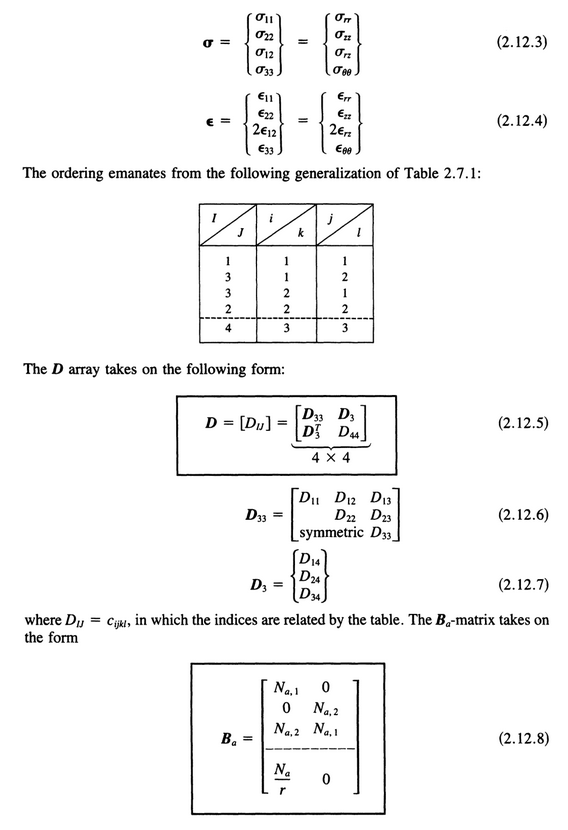
\includegraphics[width=10cm]{images/axisymmetry/hughes1}
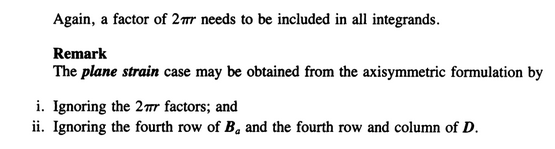
\includegraphics[width=10cm]{images/axisymmetry/hughes2}\\
{\captionfont Taken from pages 101 of \fullcite{hugh}.}
\end{center}


Also check page 469 of Gresho \& Sani's book, and 
see their remark on axisymmetric case for the N-S equations on page 545.

\Literature:
\begin{itemize}
\item \fullcite{taba96}
\item \fullcite{ruas03}
\item \fullcite{leli12} 
\item \fullcite{pric03}
\end{itemize}




